\documentclass[10pt,aspectratio=169]{beamer}


\usepackage[T1]{fontenc}
\usepackage[utf8]{inputenc}
\usepackage{lmodern}
\usepackage{microtype}
\usepackage{amsmath,amssymb}
\usepackage{booktabs}
\usepackage{array}
\usepackage{tabularx}
\usepackage{graphicx}
\usepackage{tikz}
\usetikzlibrary{arrows.meta,positioning,calc,shapes.geometric}
\usepackage{pgfplots}
\pgfplotsset{compat=1.18}
\usepackage{hyperref}

\graphicspath{{images/}}

\definecolor{RoutlyBlue}{RGB}{65,105,225}
\definecolor{RoutlyPurple}{RGB}{132,126,245}
\definecolor{RoutlyMagenta}{RGB}{235,0,118}
\definecolor{RoutlyCyan}{RGB}{53,174,190}
\definecolor{RoutlyGreen}{RGB}{30,155,90}
\definecolor{RoutlyOrange}{RGB}{246,128,35}
\definecolor{RoutlyRed}{RGB}{218,66,77}
\definecolor{RoutlyInk}{RGB}{29,32,38}
\definecolor{RoutlyMuted}{RGB}{102,108,118}
\definecolor{RoutlyPaleBlue}{RGB}{235,244,251}
\definecolor{RoutlyPalePurple}{RGB}{241,240,255}
\definecolor{RoutlyPaleOrange}{RGB}{255,245,232}
\definecolor{RoutlyPaleGreen}{RGB}{235,248,241}
\definecolor{RoutlyPaleRed}{RGB}{255,238,239}
\definecolor{RoutlyRule}{RGB}{205,210,218}

\usetheme{default}
\usefonttheme{professionalfonts}
\setbeamercolor{normal text}{fg=RoutlyInk,bg=white}
\setbeamercolor{frametitle}{fg=RoutlyInk,bg=white}
\setbeamerfont{frametitle}{size=\Large,series=\mdseries}
\setbeamerfont{title}{size=\LARGE,series=\mdseries}
\setbeamerfont{subtitle}{size=\normalsize,shape=\itshape}
\setbeamerfont{footline}{size=\tiny}
\setbeamertemplate{navigation symbols}{}
\setbeamersize{text margin left=0.58cm,text margin right=0.58cm}
\setbeamertemplate{items}[square]
\setbeamercolor{itemize item}{fg=RoutlyBlue}
\setbeamercolor{itemize subitem}{fg=RoutlyPurple}
\setlength{\leftmargini}{1.25em}
\setlength{\leftmarginii}{1.10em}

\setbeamertemplate{frametitle}{%
  \vspace{0.16cm}\insertframetitle\par
  \vspace{0.10cm}
}

\setbeamercolor{foot left}{fg=white,bg=RoutlyBlue}
\setbeamercolor{foot centre}{fg=RoutlyMagenta,bg=RoutlyPalePurple}
\setbeamercolor{foot right}{fg=RoutlyInk,bg=RoutlyPalePurple}
\setbeamertemplate{footline}{%
  \leavevmode%
  \hbox{%
    \begin{beamercolorbox}[wd=.42\paperwidth,ht=2.35ex,dp=0.8ex,leftskip=.22cm]{foot left}%
      S. Cozza, F. Cristiano, E. Ielpa, G. Rudi \quad (University of Calabria)
    \end{beamercolorbox}%
    \begin{beamercolorbox}[wd=.24\paperwidth,ht=2.35ex,dp=0.8ex,center]{foot centre}%
      \textbf{Routly Planner}
    \end{beamercolorbox}%
    \begin{beamercolorbox}[wd=.34\paperwidth,ht=2.35ex,dp=0.8ex,rightskip=.22cm plus 1fil]{foot right}%
      July 2026 \hfill \insertframenumber\,/\,\inserttotalframenumber
    \end{beamercolorbox}%
  }%
}

\setbeamertemplate{caption}{\raggedright\insertcaption\par}
\setbeamerfont{caption}{size=\scriptsize}
\setbeamercolor{caption name}{fg=RoutlyBlue}

\newcommand{\takeaway}[1]{%
  \begin{beamercolorbox}[rounded=true,sep=0.65ex,wd=\linewidth]{normal text}%
    \textbf{Takeaway:} #1
  \end{beamercolorbox}%
}

\newcommand{\smallsource}[1]{%
  \par\vspace{0.15ex}{\tiny\color{RoutlyMuted}#1}%
}

\newcommand{\metric}[3]{%
  \begin{beamercolorbox}[rounded=true,sep=0.75ex,wd=\linewidth]{#1}%
    {\Large\bfseries #2}\par
    {\scriptsize #3}
  \end{beamercolorbox}%
}

\setbeamercolor{metric blue}{fg=RoutlyInk,bg=RoutlyPaleBlue}
\setbeamercolor{metric purple}{fg=RoutlyInk,bg=RoutlyPalePurple}
\setbeamercolor{metric orange}{fg=RoutlyInk,bg=RoutlyPaleOrange}
\setbeamercolor{metric green}{fg=RoutlyInk,bg=RoutlyPaleGreen}
\setbeamercolor{metric red}{fg=RoutlyInk,bg=RoutlyPaleRed}

\title{Routly: Scalable PDDL+ Urban Routing}
\subtitle{Model simplification, controller-based replanning, and LLM road events}
\author{S. Cozza \quad F. Cristiano \quad E. Ielpa \quad G. Rudi}
\institute{University of Calabria\\Artificial Intelligence and Computer Science}
\date{July 2026}

% Notes are included for rehearsal but hidden in the normal PDF.
% Replace "hide notes" with "show notes on second screen=right" if desired.
\setbeameroption{hide notes}

\begin{document}

% 1 ---------------------------------------------------------------------------
\begin{frame}[plain]
  \centering
  \vspace{1.2cm}
  {\usebeamerfont{title}\inserttitle\par}
  \vspace{0.28cm}
  {\usebeamerfont{subtitle}\insertsubtitle\par}
  \vspace{0.75cm}
  {\normalsize\insertauthor\par}
  \vspace{0.45cm}
  {\small\insertinstitute\par}
  \vfill
  {\small\insertdate\par}
  \vspace{0.75cm}
  \note{Time: 15 seconds. Introduce Routly as an urban routing framework over real road networks. State the three themes that structure the talk: richer PDDL+ modelling, two complementary scalability strategies, and validated LLM-generated disruptions.}
\end{frame}

% 2 ---------------------------------------------------------------------------
\begin{frame}{Problem \& Goal}
  \begin{columns}[T,onlytextwidth]
    \begin{column}{0.57\textwidth}
      \textbf{Input:} a directed road graph $G=(L,R)$, a vehicle $v$, start $s$, and goal $g$.

      \vspace{0.30cm}
      \setbeamercolor{block title}{fg=RoutlyInk,bg=RoutlyPaleBlue}
      \setbeamercolor{block body}{fg=RoutlyInk,bg=RoutlyPaleBlue}
      \begin{beamerboxesrounded}[upper=block title,lower=block body,shadow=true]{Planning objective}
        Find a minimum-cost route while respecting:
        \begin{itemize}
          \item road availability and disruptions;
          \item traffic-dependent travel time;
          \item traffic-light delay;
          \item optional fuel and refuelling constraints.
        \end{itemize}
      \end{beamerboxesrounded}

      \vspace{0.25cm}
      \textbf{Core challenge:} realistic features make the decision model useful, but rapidly increase the symbolic and numeric planning cost.
    \end{column}
    \begin{column}{0.40\textwidth}
      \centering
      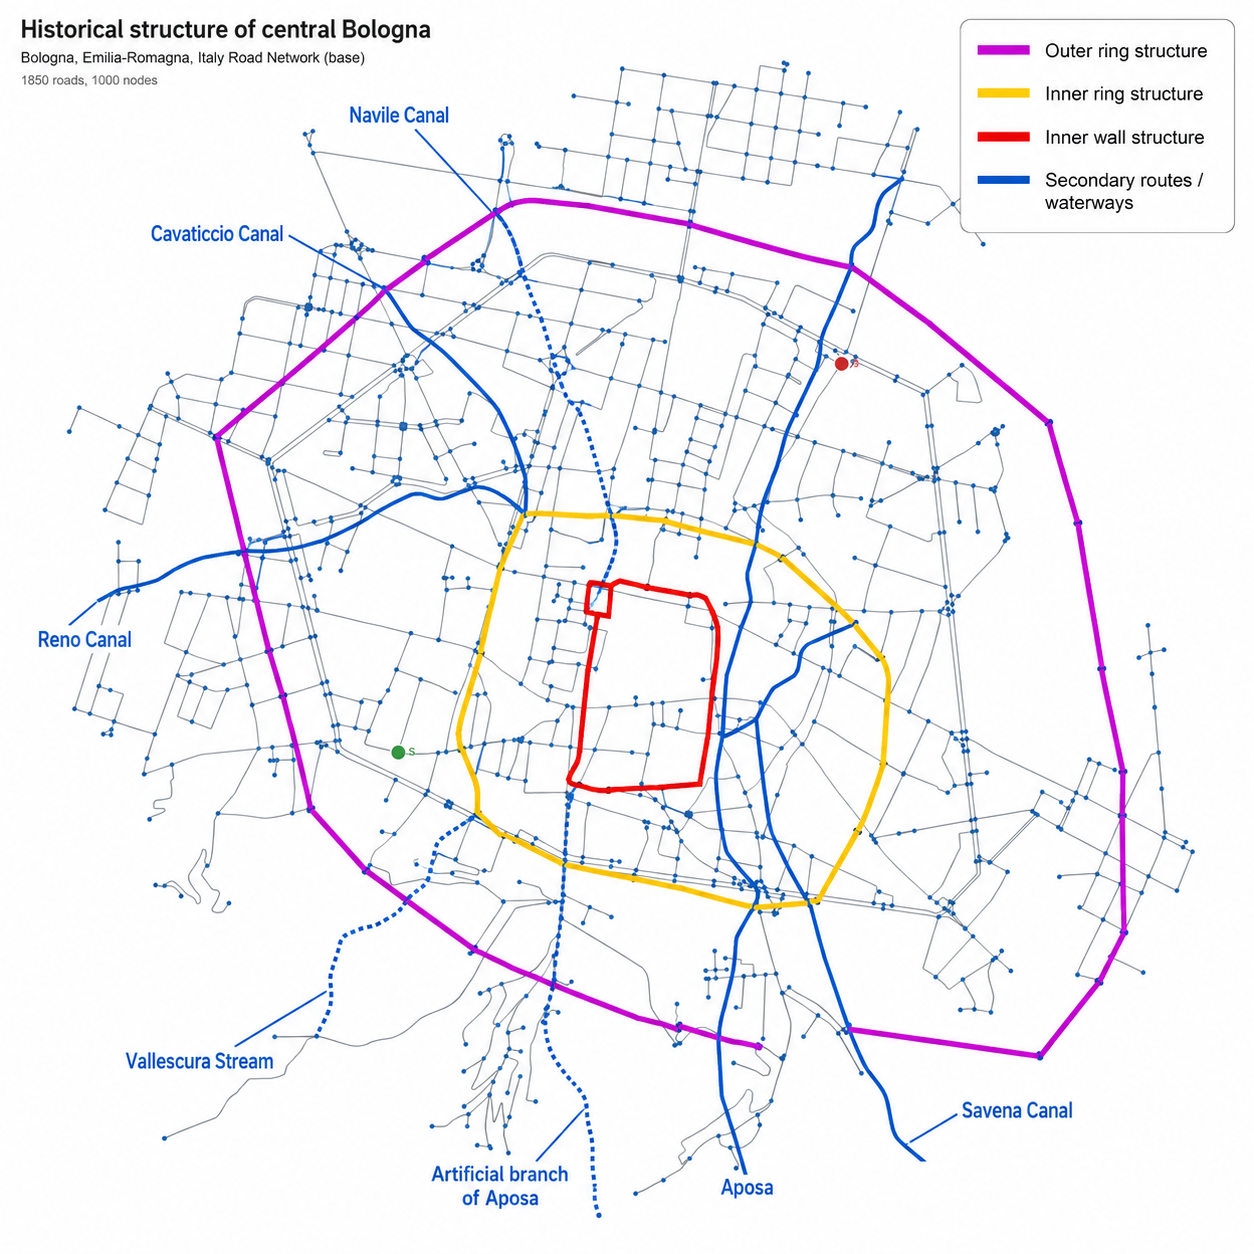
\includegraphics[width=0.84\linewidth,height=0.67\textheight,keepaspectratio]{bologna_urban_structure.png}
      \smallsource{Bologna case study: radial corridors, a ring structure, and dense alternatives.}
    \end{column}
  \end{columns}
  \note{Time: 30 seconds. Define the input graph, vehicle, start, and goal. The route must minimise a numeric cost while respecting road availability, time, traffic lights, and optional fuel. Close with the main tension: richer modelling gives more realistic decisions but a much larger planning problem.}
\end{frame}

% 3 ---------------------------------------------------------------------------
\begin{frame}{Why PDDL+?}
  \textbf{Routly does not claim to replace specialised shortest-path algorithms.}

  \vspace{0.18cm}
  \centering
  {\small
  \begin{tabularx}{0.92\linewidth}{@{}>{\bfseries}p{2.75cm}XX@{}}
    \toprule
    Aspect & Graph routing & PDDL/PDDL+ \\
    \midrule
    Typical objective & shortest or fastest path & logical goal with a numeric metric \\
    Time-dependent costs & dedicated algorithms & numeric fluents, processes, events, windows \\
    Resources and rules & task-specific extensions & expressed in the same domain \\
    Scalability & very high on the specialised task & strongly depends on encoding and grounding \\
    \bottomrule
  \end{tabularx}}

  \vspace{0.20cm}
  \begin{columns}[T,onlytextwidth]
    \begin{column}{0.32\textwidth}
      \metric{metric blue}{Actions}{controlled decisions}
    \end{column}
    \begin{column}{0.32\textwidth}
      \metric{metric purple}{Processes}{continuous evolution}
    \end{column}
    \begin{column}{0.32\textwidth}
      \metric{metric orange}{Events}{autonomous changes}
    \end{column}
  \end{columns}

  \vspace{0.18cm}
  \takeaway{PDDL+ offers one declarative language for heterogeneous constraints; the price is sensitivity to model granularity and grounding.}
  \note{Time: 35 seconds. Acknowledge that Dijkstra, A-star, and time-dependent routing are excellent at their specialised task. Routly uses PDDL+ because actions, processes, events, numeric resources, and logical constraints can coexist in one domain. The contribution is scalable declarative modelling, not a universal replacement for graph algorithms.}
\end{frame}

% 4 ---------------------------------------------------------------------------
\begin{frame}{Research Questions \& Contributions}
  \setbeamercolor{block title}{fg=RoutlyInk,bg=RoutlyPalePurple}
  \setbeamercolor{block body}{fg=RoutlyInk,bg=RoutlyPalePurple}
  \begin{beamerboxesrounded}[upper=block title,lower=block body,shadow=true]{RQ1 - Model-side scalability}
    How much do compilation, alternative state representations, hybrid time modelling, and road abstraction reduce grounding and planning cost?
  \end{beamerboxesrounded}

  \vspace{0.18cm}
  \setbeamercolor{block title}{fg=RoutlyInk,bg=RoutlyPaleBlue}
  \setbeamercolor{block body}{fg=RoutlyInk,bg=RoutlyPaleBlue}
  \begin{beamerboxesrounded}[upper=block title,lower=block body,shadow=true]{RQ2 - Controller-side scalability}
    Can Python preserve the detailed process model while building a valid trip from smaller congestion or fuel plans?
  \end{beamerboxesrounded}

  \vspace{0.18cm}
  \setbeamercolor{block title}{fg=RoutlyInk,bg=RoutlyPaleOrange}
  \setbeamercolor{block body}{fg=RoutlyInk,bg=RoutlyPaleOrange}
  \begin{beamerboxesrounded}[upper=block title,lower=block body,shadow=true]{RQ3 - LLM event quality}
    Can an LLM generate valid, relevant disruptions without seeing the baseline route, while ENHSP remains responsible for planning?
  \end{beamerboxesrounded}

  \vspace{0.28cm}
  \centering
  \textbf{Two scalability branches + one independent robustness experiment}
  \note{Time: 30 seconds. Present the three research questions as the structure of the talk. RQ1 changes the model given to ENHSP. RQ2 changes how ENHSP is called while preserving the process model. RQ3 is separate: it tests route adaptation under validated plan-hidden events.}
\end{frame}

% 3 ---------------------------------------------------------------------------
\begin{frame}{Data \& Planning Pipeline}
  \textbf{Same physical network, progressively richer planning representations.}

  \vspace{0.25cm}
  \centering
  
\begin{tikzpicture}[
    node distance=0.30cm,
    box/.style={draw=RoutlyRule,rounded corners=3pt,fill=white,minimum height=0.82cm,minimum width=2.02cm,align=center,font=\scriptsize},
    arr/.style={-{Latex[length=2mm]},thick,draw=RoutlyBlue}
  ]
    \node[box] (osm) {OpenStreetMap\\OSMnx};
    \node[box,right=of osm] (filter) {crop, connect,\\cap nodes};
    \node[box,right=of filter] (macro) {optional\\macro-roads};
    \node[box,right=of macro] (pddl) {PDDL/PDDL+\\generation};
    \node[box,right=of pddl] (enhsp) {ENHSP\\plan};
    \node[box,right=of enhsp] (sumo) {SUMO\\validation};
    \draw[arr] (osm) -- (filter);
    \draw[arr] (filter) -- (macro);
    \draw[arr] (macro) -- (pddl);
    \draw[arr] (pddl) -- (enhsp);
    \draw[arr] (enhsp) -- (sumo);
  \end{tikzpicture}

  \vspace{0.22cm}
  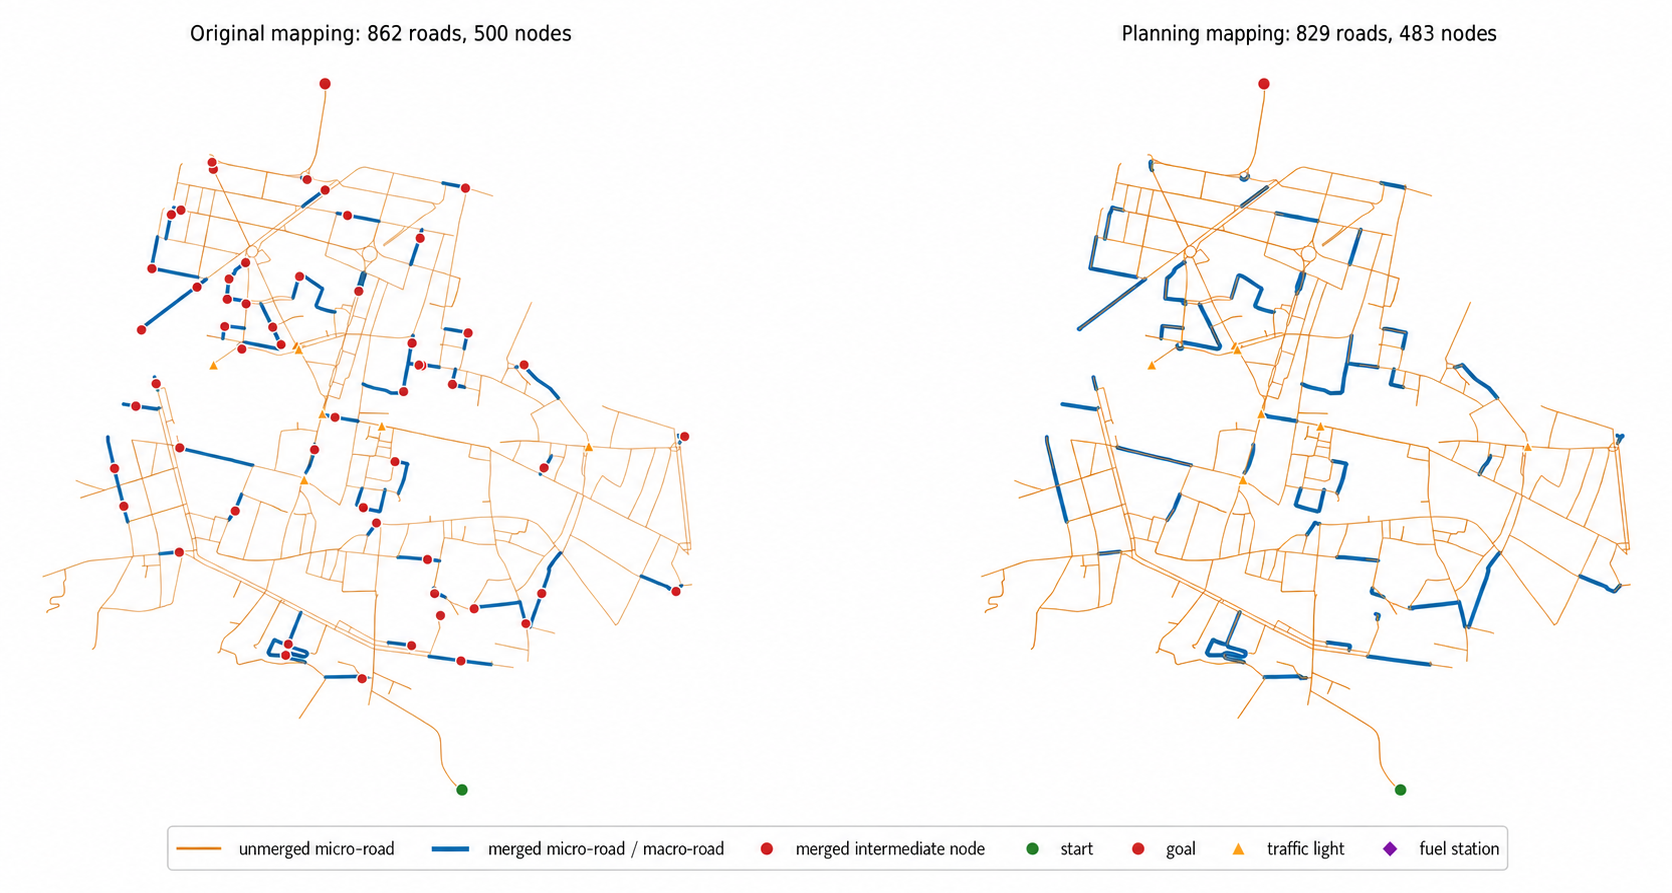
\includegraphics[width=0.77\linewidth,height=0.52\textheight,keepaspectratio]{macro_roads_comparison.png}

  \vspace{-0.15cm}
  \begin{columns}[T,onlytextwidth]
    \begin{column}{0.50\textwidth}
      {\scriptsize\textbf{Reproducibility:} radius, node cap, seed, features, planner mode, and experiment outputs are controlled by validated YAML.}
    \end{column}
    \begin{column}{0.47\textwidth}
      {\scriptsize\textbf{Role separation:} ENHSP decides; SUMO executes and visualises the expanded micro-road route.}
    \end{column}
  \end{columns}
  \note{Time: 35 seconds. Walk left to right through the pipeline. OSMnx builds and simplifies the drivable graph, project preprocessing limits the experimental instance, optional macro-roads remove non-decision chains, ENHSP solves the generated planning problem, and SUMO validates the expanded route. Mention that each run saves its YAML snapshot.}
\end{frame}

% 4 ---------------------------------------------------------------------------
\begin{frame}{Model Roadmap}
  \centering
  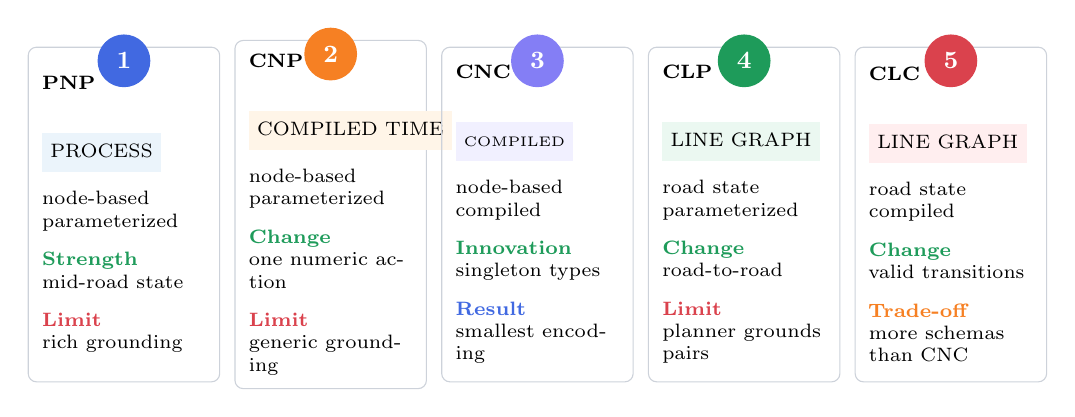
\begin{tikzpicture}[
    card/.style={draw=RoutlyRule,rounded corners=3pt,minimum width=2.36cm,minimum height=4.25cm,align=left,text width=2.08cm,inner sep=5pt,font=\scriptsize},
    badge/.style={circle,text=white,font=\bfseries\small,minimum size=0.67cm},
    group/.style={draw,densely dotted,rounded corners=3pt,inner sep=5pt}
  ]
    \node[card] (pnp) at (0,0) {\vspace{0.52cm}\textbf{PNP}\par\colorbox{RoutlyPaleBlue}{\strut PROCESS}\par\medskip node-based\par parameterized\par\medskip\textcolor{RoutlyGreen}{\textbf{Strength}}\par mid-road state\par\medskip\textcolor{RoutlyRed}{\textbf{Limit}}\par rich grounding};
    \node[badge,fill=RoutlyBlue] at ($(pnp.north)+(0,-0.18)$) {1};

    \node[card,right=0.18cm of pnp] (cnp) {\vspace{0.52cm}\textbf{CNP}\par\colorbox{RoutlyPaleOrange}{\strut COMPILED TIME}\par\medskip node-based\par parameterized\par\medskip\textcolor{RoutlyGreen}{\textbf{Change}}\par one numeric action\par\medskip\textcolor{RoutlyRed}{\textbf{Limit}}\par generic grounding};
    \node[badge,fill=RoutlyOrange] at ($(cnp.north)+(0,-0.18)$) {2};

    \node[card,right=0.18cm of cnp] (cnc) {\vspace{0.52cm}\textbf{CNC}\par\colorbox{RoutlyPalePurple}{\strut\tiny COMPILED}\par\medskip node-based\par compiled\par\medskip\textcolor{RoutlyGreen}{\textbf{Innovation}}\par singleton types\par\medskip\textcolor{RoutlyBlue}{\textbf{Result}}\par smallest encoding};
    \node[badge,fill=RoutlyPurple] at ($(cnc.north)+(0,-0.18)$) {3};

    \node[card,right=0.18cm of cnc] (clp) {\vspace{0.52cm}\textbf{CLP}\par\colorbox{RoutlyPaleGreen}{\strut LINE GRAPH}\par\medskip road state\par parameterized\par\medskip\textcolor{RoutlyGreen}{\textbf{Change}}\par road-to-road\par\medskip\textcolor{RoutlyRed}{\textbf{Limit}}\par planner grounds pairs};
    \node[badge,fill=RoutlyGreen] at ($(clp.north)+(0,-0.18)$) {4};

    \node[card,right=0.18cm of clp] (clc) {\vspace{0.52cm}\textbf{CLC}\par\colorbox{RoutlyPaleRed}{\strut LINE GRAPH}\par\medskip road state\par compiled\par\medskip\textcolor{RoutlyGreen}{\textbf{Change}}\par valid transitions\par\medskip\textcolor{RoutlyOrange}{\textbf{Trade-off}}\par more schemas than CNC};
    \node[badge,fill=RoutlyRed] at ($(clc.north)+(0,-0.18)$) {5};
  \end{tikzpicture}

  \vspace{0.18cm}
  \begin{tabular}{@{}ccc@{}}
    \toprule
    \textbf{Traversal model} & \textbf{State representation} & \textbf{Action generation} \\
    process / compiled duration & node-based / line graph & parameterized / compiled \\
    \bottomrule
  \end{tabular}

  \vspace{0.12cm}
  {\scriptsize These are independent modelling axes: the line graph is an alternative representation, not an automatically better final step.}
  \note{Time: 35 seconds. Start from the expressive PDDL+ baseline. Compiled duration removes process and event state but not generic grounding. Compiled action generation moves valid instantiation to Python through singleton types. Line graph changes the state from nodes to roads and is tested in both parameterized and compiled forms. Stress that the axes are independent.}
\end{frame}

% 7 ---------------------------------------------------------------------------
\begin{frame}{Traversal Model: Process vs Compiled Duration}
  \textbf{Modelling question: do we need to observe the vehicle while it is inside a road?}

  \vspace{0.28cm}
  \begin{columns}[T,onlytextwidth]
    \begin{column}{0.49\textwidth}
      \setbeamercolor{block title}{fg=white,bg=RoutlyBlue}
      \setbeamercolor{block body}{fg=RoutlyInk,bg=RoutlyPaleBlue}
      \begin{beamerboxesrounded}[upper=block title,lower=block body,shadow=true]{PDDL+ process baseline}
        \centering
        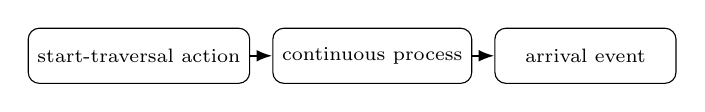
\begin{tikzpicture}[node distance=0.28cm,font=\scriptsize]
          \node[draw,rounded corners,fill=white,minimum width=2.3cm,minimum height=0.7cm] (a) {start-traversal action};
          \node[draw,rounded corners,fill=white,minimum width=2.3cm,minimum height=0.7cm,right=of a] (p) {continuous process};
          \node[draw,rounded corners,fill=white,minimum width=2.3cm,minimum height=0.7cm,right=of p] (e) {arrival event};
          \draw[-{Latex[length=2mm]},thick] (a) -- (p);
          \draw[-{Latex[length=2mm]},thick] (p) -- (e);
        \end{tikzpicture}

        \vspace{0.22cm}
        \scriptsize
        \begin{itemize}
          \item preserves mid-road distance and speed;
          \item supports continuous fuel consumption;
          \item expressive, but exposes rich parameter combinations.
        \end{itemize}
      \end{beamerboxesrounded}
    \end{column}
    \begin{column}{0.49\textwidth}
      \setbeamercolor{block title}{fg=white,bg=RoutlyOrange}
      \setbeamercolor{block body}{fg=RoutlyInk,bg=RoutlyPaleOrange}
      \begin{beamerboxesrounded}[upper=block title,lower=block body,shadow=true]{Compiled duration}
        \centering
        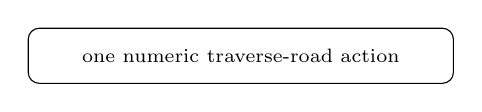
\begin{tikzpicture}[font=\scriptsize]
          \node[draw,rounded corners,fill=white,minimum width=5.4cm,minimum height=0.7cm] {one numeric traverse-road action};
        \end{tikzpicture}

        \vspace{0.22cm}
        \scriptsize
        \begin{itemize}
          \item Python precomputes road traversal duration;
          \item no process, arrival event, or mid-road fluents;
          \item semantic simplification, but generic grounding remains.
        \end{itemize}
      \end{beamerboxesrounded}
    \end{column}
  \end{columns}

  \vspace{0.30cm}
  \centering\scriptsize
  \begin{tabular}{@{}lcc@{}}
    \toprule
    Core encoding feature & Process & Compiled duration \\
    \midrule
    Movement mechanisms & 3 & 1 \\
    Mid-road vehicle fluents & 2 & 0 \\
    Loose grounding exposure before action compilation & $4.255\times10^9$ & $4.255\times10^9$ \\
    \bottomrule
  \end{tabular}

  \vspace{0.20cm}
  \takeaway{Compiled duration removes unnecessary semantics, but action generation must also change to solve the grounding bottleneck.}
  \note{Time: 35 seconds. Contrast the three-mechanism process encoding with one compiled numeric action. The compiled model is enough when only node-to-node route choice matters. However, the table shows that the parameter space is still the same if ENHSP must ground one generic road-location-location action.}
\end{frame}

% 8 ---------------------------------------------------------------------------
\begin{frame}{State \& Action Generation: Where Grounding Happens}
  \begin{columns}[T,onlytextwidth]
    \begin{column}{0.49\textwidth}
      \textbf{State representation}

      \vspace{0.20cm}
      \metric{metric blue}{Node-based}{vehicle at a location; action selects road, from, and to}
      \vspace{0.15cm}
      \centering
      $|R||L|^2|W|\;\approx\;4.255\times10^9$

      \vspace{0.28cm}
      \metric{metric green}{Line graph}{vehicle ready on a road; action selects the successor road}
      \vspace{0.15cm}
      \centering
      $|R|^2|W|\;\approx\;1.443\times10^7$
    \end{column}
    \begin{column}{0.49\textwidth}
      \textbf{Action generation}

      \vspace{0.20cm}
      \setbeamercolor{block title}{fg=RoutlyInk,bg=RoutlyPaleOrange}
      \setbeamercolor{block body}{fg=RoutlyInk,bg=RoutlyPaleOrange}
      \begin{beamerboxesrounded}[upper=block title,lower=block body,shadow=true]{Parameterized}
        \scriptsize One compact action schema; ENHSP receives the Cartesian product and filters invalid combinations.
      \end{beamerboxesrounded}

      \vspace{0.22cm}
      \setbeamercolor{block title}{fg=RoutlyInk,bg=RoutlyPalePurple}
      \setbeamercolor{block body}{fg=RoutlyInk,bg=RoutlyPalePurple}
      \begin{beamerboxesrounded}[upper=block title,lower=block body,shadow=true]{Compiled + singleton types}
        \scriptsize Python emits only valid road/location/window schemas. Each parameter type contains one compatible object.
        \[
          N_{\mathrm{node,compiled}}=S+D|W|=1769
        \]
      \end{beamerboxesrounded}
    \end{column}
  \end{columns}

  \vspace{0.32cm}
  \takeaway{A compact domain file can still be expensive. Routly trades a larger generated domain for dramatically less planner-side grounding.}
  \note{Time: 30 seconds. Explain that node-based generic actions multiply roads by two location parameters and time windows. Line graph reduces arity but still leaves filtering to ENHSP. Compiled generation is different: Python already knows the topology and emits only valid schemas, with singleton types preserving compatibility with ENHSP's grounding mechanism.}
\end{frame}

% 9 ---------------------------------------------------------------------------
\begin{frame}{Realistic Base Domain}
  \begin{columns}[T,onlytextwidth]
    \begin{column}{0.49\textwidth}
      \setbeamercolor{block title}{fg=RoutlyInk,bg=RoutlyPaleBlue}
      \setbeamercolor{block body}{fg=RoutlyInk,bg=RoutlyPaleBlue}
      \begin{beamerboxesrounded}[upper=block title,lower=block body,shadow=true]{Traffic lights}
        \scriptsize Junctions are simple, medium, or complex from degree and highest road class.
        \[
          d^{\mathrm{signal}}=\frac{r^2}{2(g+y+r)}
        \]
      \end{beamerboxesrounded}

      \vspace{0.18cm}
      \setbeamercolor{block title}{fg=RoutlyInk,bg=RoutlyPaleGreen}
      \setbeamercolor{block body}{fg=RoutlyInk,bg=RoutlyPaleGreen}
      \begin{beamerboxesrounded}[upper=block title,lower=block body,shadow=true]{Fuel}
        \scriptsize Limited tank, discrete or continuous consumption, OSM or seeded synthetic stations, and optional refuelling controller.
      \end{beamerboxesrounded}
    \end{column}
    \begin{column}{0.49\textwidth}
      \setbeamercolor{block title}{fg=RoutlyInk,bg=RoutlyPaleOrange}
      \setbeamercolor{block body}{fg=RoutlyInk,bg=RoutlyPaleOrange}
      \begin{beamerboxesrounded}[upper=block title,lower=block body,shadow=true]{Congestion}
        \scriptsize Background traffic produces class-dependent costs:
        \[
          c_r=\min\!\left(2,1+\frac{n_r}{\tau_{\mathrm{class}}}\right),\quad
          \tau=(20,35,50).
        \]
        \scriptsize Static, dynamic, or hybrid; hybrid retains time only when $\max c_{r,w}-\min c_{r,w}\ge 0.10$.
      \end{beamerboxesrounded}

      \vspace{0.18cm}
      \setbeamercolor{block title}{fg=RoutlyInk,bg=RoutlyPaleRed}
      \setbeamercolor{block body}{fg=RoutlyInk,bg=RoutlyPaleRed}
      \begin{beamerboxesrounded}[upper=block title,lower=block body,shadow=true]{Road disruptions}
        \scriptsize Closures change logical availability; slowdowns increase congestion and therefore traversal duration.
      \end{beamerboxesrounded}
    \end{column}
  \end{columns}

  \vspace{0.28cm}
  \takeaway{Realism is useful, but every extra object, fluent, condition, and time window increases the grounded problem.}
  \note{Time: 40 seconds. Give one sentence per feature. Traffic-light delay is precomputed as an expected wait. Congestion depends on road capacity and may vary by time window. Fuel is numeric and can be consumed discretely or continuously. Disruptions alter road availability or cost. Then connect these realistic features to the grounding bottleneck.}
\end{frame}

% 6 ---------------------------------------------------------------------------
\begin{frame}{Controller-Side Scalability}
  \textbf{Keep the expressive process model; decompose the horizon in Python.}

  \vspace{0.18cm}
  \centering
  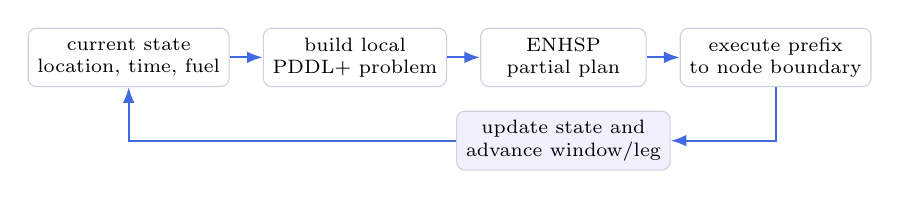
\begin{tikzpicture}[
    node distance=0.42cm,
    box/.style={draw=RoutlyRule,rounded corners=3pt,fill=white,minimum height=0.74cm,minimum width=2.10cm,align=center,font=\scriptsize},
    arr/.style={-{Latex[length=2mm]},thick,draw=RoutlyBlue}
  ]
    \node[box] (state) {current state\\location, time, fuel};
    \node[box,right=of state] (problem) {build local\\PDDL+ problem};
    \node[box,right=of problem] (plan) {ENHSP\\partial plan};
    \node[box,right=of plan] (prefix) {execute prefix\\to node boundary};
    \node[box,below=0.30cm of plan,fill=RoutlyPalePurple] (update) {update state and\\advance window/leg};
    \draw[arr] (state) -- (problem);
    \draw[arr] (problem) -- (plan);
    \draw[arr] (plan) -- (prefix);
    \draw[arr] (prefix.south) |- (update.east);
    \draw[arr] (update.west) -| (state.south);
  \end{tikzpicture}

  \vspace{0.12cm}
  \begin{columns}[T,onlytextwidth]
    \begin{column}{0.49\textwidth}
      \centering
      \textbf{Congestion controller}\par
      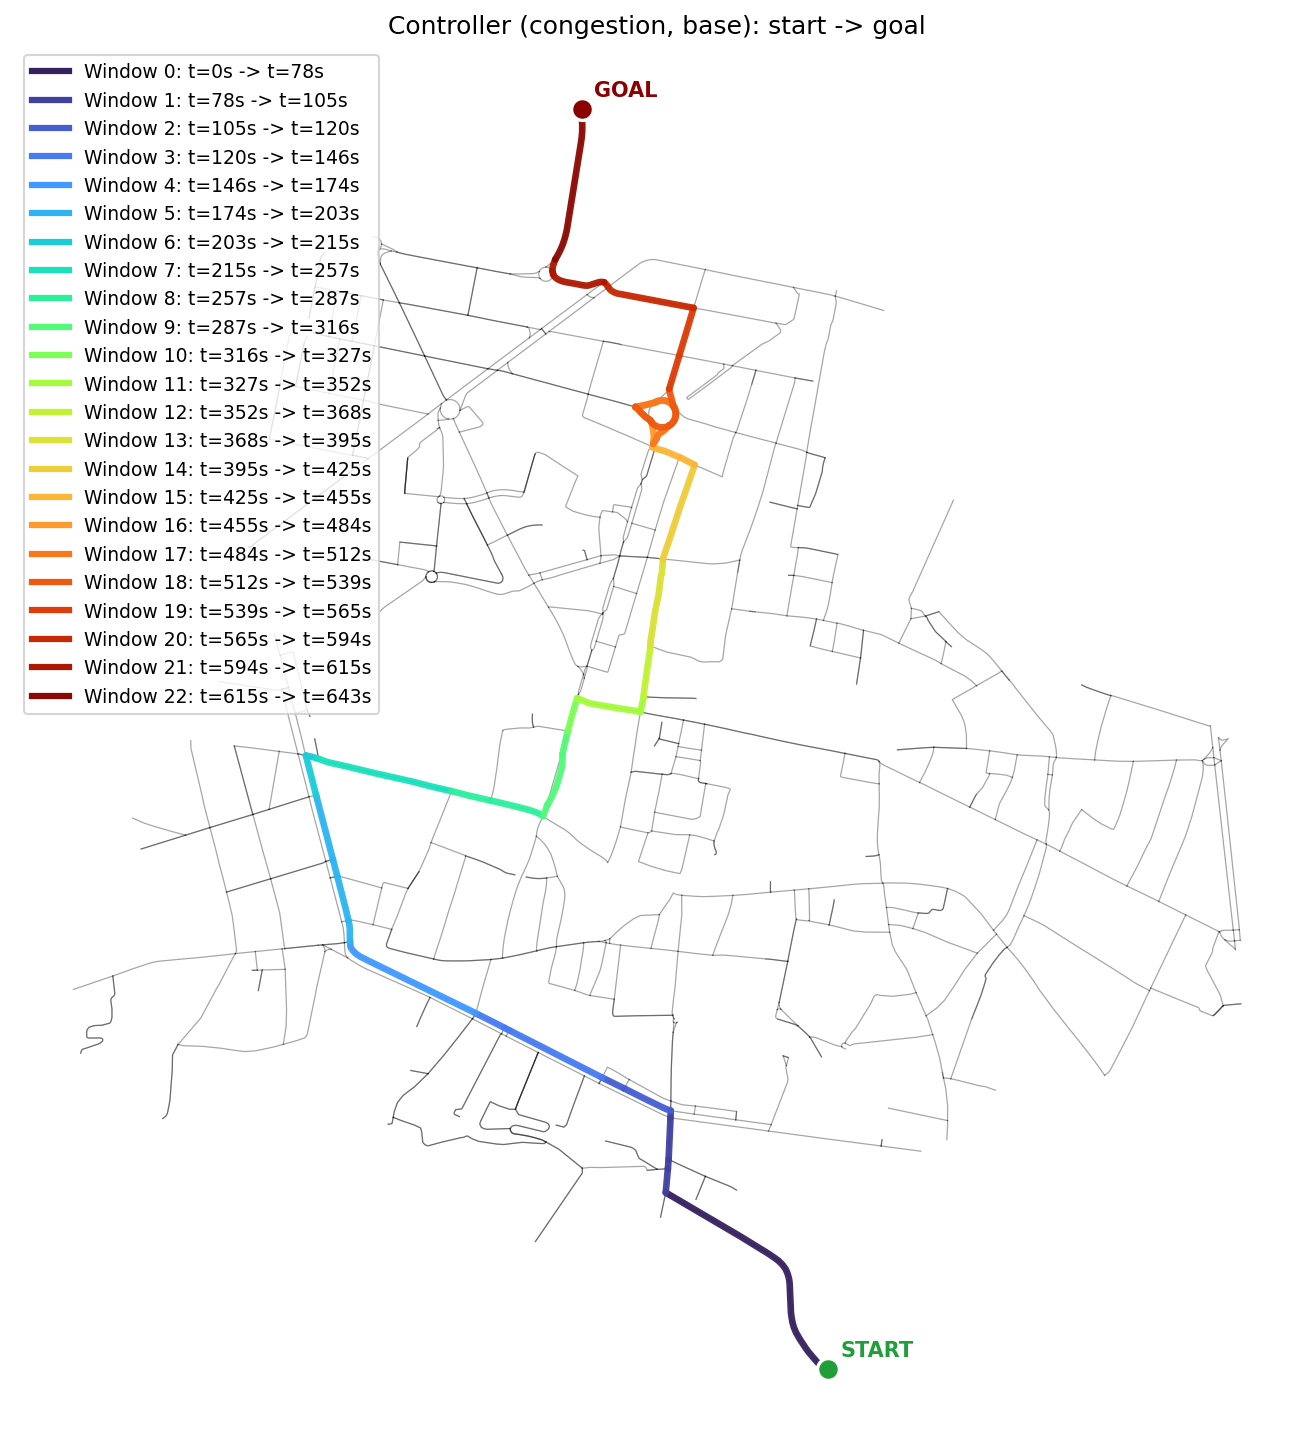
\includegraphics[height=0.37\textheight,width=0.93\linewidth,keepaspectratio]{congestion_controller_500.png}
      {\scriptsize Snapshot per window; reuse cached plans when costs are unchanged.}
    \end{column}
    \begin{column}{0.49\textwidth}
      \centering
      \textbf{Fuel controller}\par
      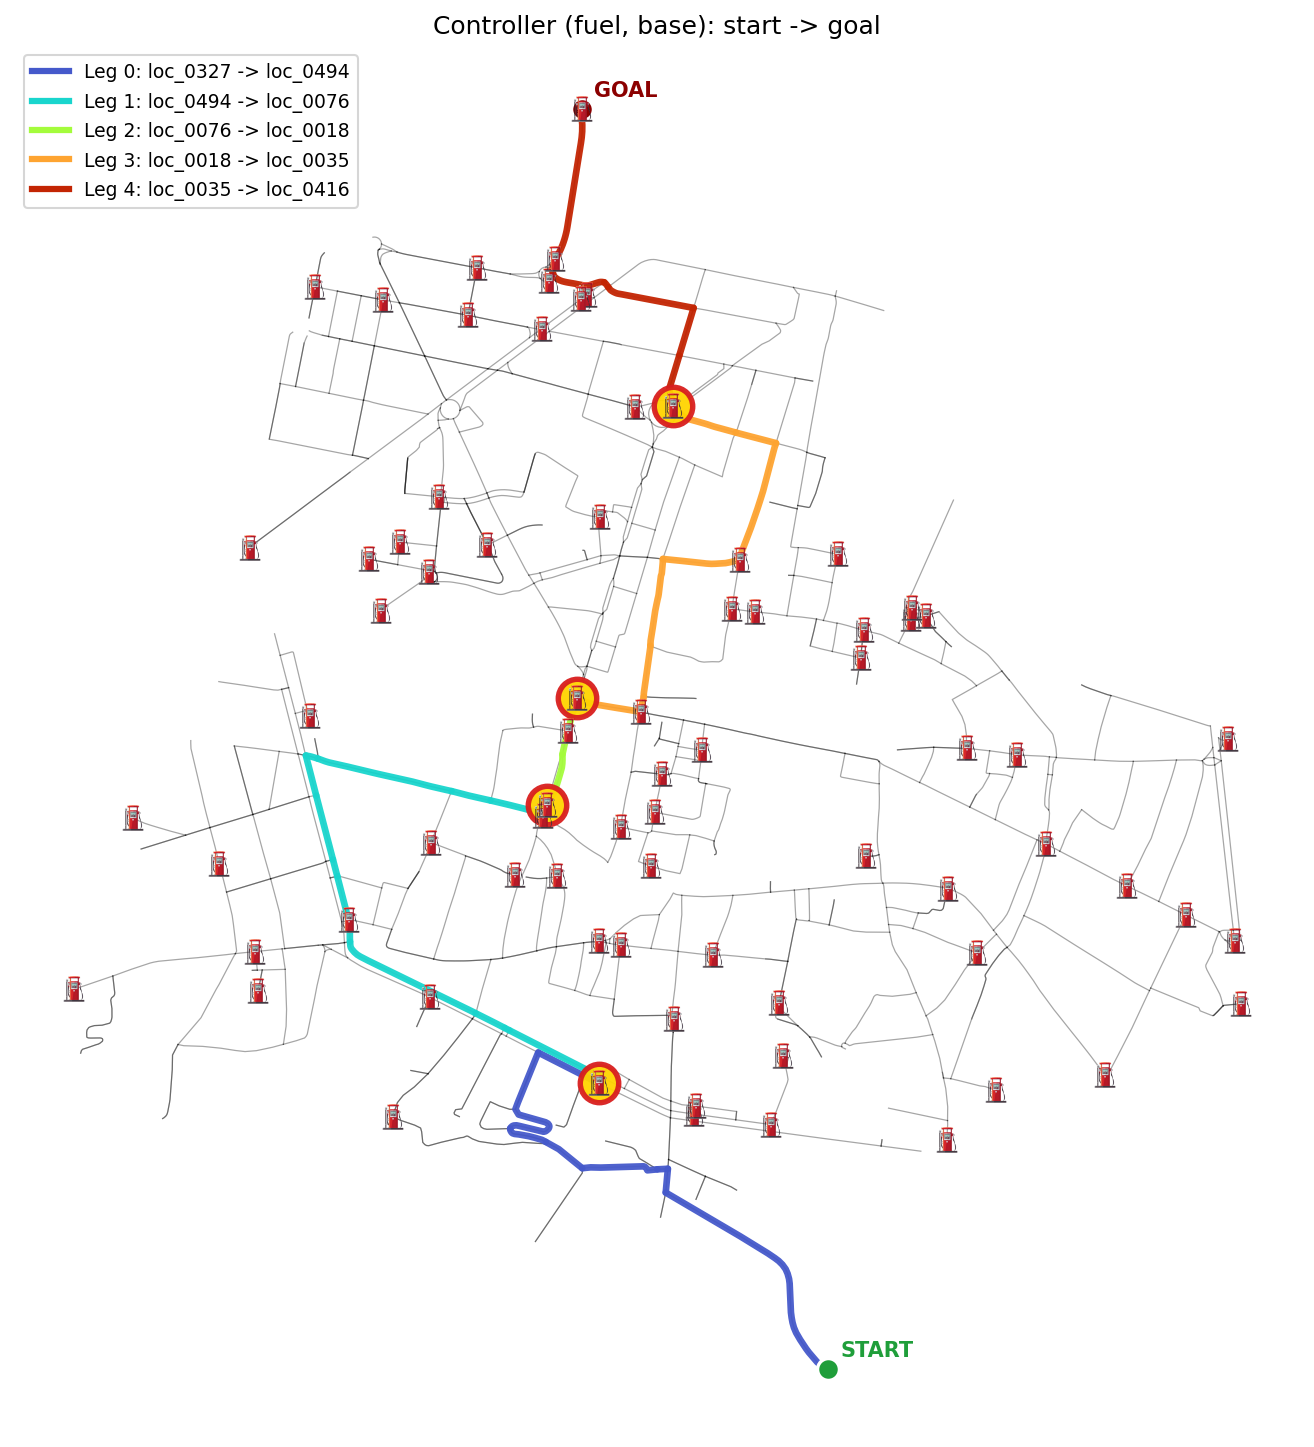
\includegraphics[height=0.37\textheight,width=0.93\linewidth,keepaspectratio]{fuel_controller_500.png}
      {\scriptsize Goal if reachable; otherwise a fuel station becomes the target.}
    \end{column}
  \end{columns}
  \note{Time: 40 seconds. Explain the common loop. Each partial plan ends at a node boundary so the process state does not need to be serialised mid-road. The congestion controller changes a static snapshot between windows and can reuse a cached plan. The fuel controller changes the temporary target according to reachability. The two controllers are currently mutually exclusive.}
\end{frame}

% 7 ---------------------------------------------------------------------------
\begin{frame}{LLM-Driven Exogenous Events}
  \begin{columns}[T,onlytextwidth]
    \begin{column}{0.53\textwidth}
      \centering
      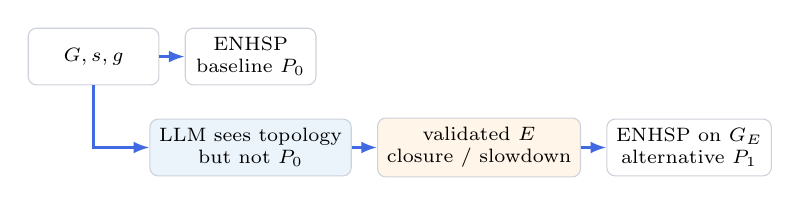
\begin{tikzpicture}[
        node distance=0.32cm,
        box/.style={draw=RoutlyRule,rounded corners=3pt,minimum height=0.72cm,minimum width=1.66cm,align=center,font=\scriptsize},
        arr/.style={-{Latex[length=2mm]},thick,draw=RoutlyBlue}
      ]
        \node[box] (g) {$G,s,g$};
        \node[box,right=of g] (p0) {ENHSP\\baseline $P_0$};
        \node[box,below=0.42cm of p0,fill=RoutlyPaleBlue] (llm) {LLM sees topology\\but not $P_0$};
        \node[box,right=of llm,fill=RoutlyPaleOrange] (event) {validated $E$\\closure / slowdown};
        \node[box,right=of event] (p1) {ENHSP on $G_E$\\alternative $P_1$};
        \draw[arr] (g) -- (p0);
        \draw[arr] (g.south) |- (llm.west);
        \draw[arr] (llm) -- (event);
        \draw[arr] (event) -- (p1);
      \end{tikzpicture}

      \vspace{0.35cm}
      \begin{itemize}
        \item The LLM proposes only structured events; it never generates the route.
        \item Strategic mode ranks up to 120 candidate roads in a start-goal corridor.
        \item Start and goal are protected; unsafe closures fall back to slowdowns.
      \end{itemize}

      \vspace{0.18cm}
      \[
        P_0=\operatorname{Plan}(G,s,g),\qquad
        P_1=\operatorname{Plan}(G_E,s,g)
      \]
    \end{column}
    \begin{column}{0.44\textwidth}
      \centering
      \includegraphics[height=0.68\textheight,width=0.96\linewidth,keepaspectratio]{500_nodes_event_map.png}
      \smallsource{Blue: baseline; green: alternative; red: closures; yellow: slowdown.}
    \end{column}
  \end{columns}
  \note{Time: 35 seconds. Make the role separation explicit: ENHSP remains the planner and the LLM is a constrained event generator. It receives topology plus start and goal, not the baseline route. Python validates events and preserves reachability. The comparison is a second planning run under a perturbed network, not yet online replanning from a moving vehicle.}
\end{frame}

% 8 ---------------------------------------------------------------------------
\begin{frame}{Results - Model-Side Scalability}
  \textbf{Fixed 300-node instance: same map, start/goal, traffic, congestion, and 8 GB heap.}

  \vspace{0.20cm}
  \begin{columns}[T,onlytextwidth]
    \begin{column}{0.69\textwidth}
      \centering
      \begin{tikzpicture}
        \begin{axis}[
          width=\linewidth,
          height=0.61\textheight,
          ybar,
          bar width=5pt,
          ymode=log,
          ymin=0.7,
          ymax=260,
          ylabel={seconds (log scale)},
          symbolic x coords={PNP,CNP,CNC,CLP,CLC},
          xtick=data,
          tick label style={font=\scriptsize},
          label style={font=\scriptsize},
          legend style={font=\scriptsize,at={(0.5,1.02)},anchor=south,legend columns=2,draw=none},
          grid=major,
          major grid style={draw=RoutlyRule},
          axis line style={draw=RoutlyMuted},
          enlarge x limits=0.15,
        ]
          \addplot[fill=RoutlyBlue,draw=RoutlyBlue] coordinates {
            (PNP,79.253) (CNP,40.379) (CNC,1.063) (CLP,76.263) (CLC,1.914)
          };
          \addplot[fill=RoutlyPurple,draw=RoutlyPurple] coordinates {
            (PNP,146.901) (CNP,41.427) (CNC,2.542) (CLP,77.464) (CLC,3.606)
          };
          \legend{Grounding,Planning}
        \end{axis}
      \end{tikzpicture}
    \end{column}
    \begin{column}{0.28\textwidth}
      \metric{metric purple}{38.0$\times$}{CNC grounding speedup vs CNP}
      \vspace{0.18cm}
      \metric{metric blue}{16.3$\times$}{CNC planning speedup vs CNP}
      \vspace{0.18cm}
      \metric{metric green}{3.605 s}{CNC total grounding + planning time}
    \end{column}
  \end{columns}

  \vspace{-0.15cm}
  \takeaway{Compilation is decisive: singleton-typed valid actions remove the generic Cartesian product. CNC remains faster than compiled line graph on the tested networks.}
  \note{Time: 40 seconds. Read the chart at a high level: the parameterized models spend tens to hundreds of seconds, while compiled action generation brings both phases close to seconds. CNC gains 38 times in grounding and 16.3 times in planning over CNP. It is also the strongest scaling configuration, reaching 2,000 requested nodes.}
\end{frame}

% 14 --------------------------------------------------------------------------
\begin{frame}{Results - Scaling from 500 to 2,000 Nodes}
  \textbf{Compiled variants with macro-road abstraction and hybrid congestion ($\theta=0.10$).}

  \vspace{0.18cm}
  \begin{columns}[T,onlytextwidth]
    \begin{column}{0.66\textwidth}
      \centering
      \begin{tikzpicture}
        \begin{axis}[
          width=\linewidth,
          height=0.61\textheight,
          xlabel={requested nodes},
          ylabel={planning time (s)},
          ymode=log,
          xmin=450,xmax=2050,
          ymin=6,ymax=700,
          xtick={500,1000,1500,2000},
          tick label style={font=\scriptsize},
          label style={font=\scriptsize},
          legend style={font=\scriptsize,at={(0.5,1.02)},anchor=south,legend columns=2,draw=none},
          grid=major,
          major grid style={draw=RoutlyRule},
          axis line style={draw=RoutlyMuted},
        ]
          \addplot[very thick,RoutlyBlue,mark=*] coordinates {
            (500,8.431) (1000,33.011) (1500,89.963) (2000,245.256)
          };
          \addplot[very thick,RoutlyPurple,mark=square*] coordinates {
            (500,16.535) (1000,103.992) (1500,299.261) (2000,489.018)
          };
          \legend{CNC node-based compiled,CLC line-graph compiled}
        \end{axis}
      \end{tikzpicture}
    \end{column}
    \begin{column}{0.31\textwidth}
      \centering\scriptsize
      \begin{tabular}{@{}rrrr@{}}
        \toprule
        Nodes & Dyn. & Static & Win. \\
        \midrule
        500  & 47  & 782  & 21 \\
        1000 & 78  & 1706 & 25 \\
        1500 & 109 & 2629 & 25 \\
        2000 & 110 & 3572 & 32 \\
        \bottomrule
      \end{tabular}

      \vspace{0.35cm}
      \metric{metric blue}{245.3 s}{CNC planning at 2,000 nodes}
      \vspace{0.18cm}
      \metric{metric purple}{489.0 s}{CLC planning at 2,000 nodes}
    \end{column}
  \end{columns}

  \vspace{-0.10cm}
  \takeaway{Both compiled formulations scale to 2,000 requested nodes; CNC is consistently faster because valid road schemas are fewer than valid road-to-road transitions.}
  \note{Time: 35 seconds. This second RQ1 experiment increases the graph size while keeping only the compiled configurations. Both reach 2,000 requested nodes. CNC remains faster at every size because the line graph duplicates a road across multiple valid successors, so compiled transitions can outnumber compiled node-based road actions.}
\end{frame}

% 15 --------------------------------------------------------------------------
\begin{frame}{Results - Controller-Side Scalability}
  \textbf{Same process + node-based + parameterized semantics; one global solve versus partial solves.}

  \vspace{0.25cm}
  \begin{columns}[T,onlytextwidth]
    \begin{column}{0.49\textwidth}
      \setbeamercolor{block title}{fg=RoutlyInk,bg=RoutlyPaleBlue}
      \setbeamercolor{block body}{fg=RoutlyInk,bg=RoutlyPaleBlue}
      \begin{beamerboxesrounded}[upper=block title,lower=block body,shadow=true]{Dynamic congestion controller}
        \centering\scriptsize
        \begin{tabular}{@{}r r r@{}}
          \toprule
          Nodes & Single-shot & Controller \\
          \midrule
          100  & 494.2 s  & \textbf{11.4 s} \\
          150  & 3238.3 s & \textbf{48.5 s} \\
          200  & \textcolor{RoutlyRed}{OOM} & 230.1 s \\
          700  & \textcolor{RoutlyRed}{OOM} & 6912.6 s \\
          1000 & \textcolor{RoutlyRed}{OOM} & Timeout \\
          \bottomrule
        \end{tabular}

        \vspace{0.20cm}
        Up to 7 cached windows at 500 nodes avoid repeated ENHSP calls.
      \end{beamerboxesrounded}
    \end{column}
    \begin{column}{0.49\textwidth}
      \setbeamercolor{block title}{fg=RoutlyInk,bg=RoutlyPaleGreen}
      \setbeamercolor{block body}{fg=RoutlyInk,bg=RoutlyPaleGreen}
      \begin{beamerboxesrounded}[upper=block title,lower=block body,shadow=true]{Fuel controller}
        \centering\scriptsize
        \begin{tabular}{@{}r r r r@{}}
          \toprule
          Nodes & Discrete & Continuous & Controller \\
          \midrule
          100  & 34.9 s & 12.6 s  & \textbf{4.9 s} \\
          150  & 58.2 s & 116.3 s & \textbf{16.7 s} \\
          200  & \textcolor{RoutlyRed}{OOM} & \textcolor{RoutlyRed}{OOM} & 167.0 s \\
          700  & \textcolor{RoutlyRed}{OOM} & \textcolor{RoutlyRed}{OOM} & 3181.1 s \\
          1000 & \textcolor{RoutlyRed}{OOM} & \textcolor{RoutlyRed}{OOM} & Timeout \\
          \bottomrule
        \end{tabular}

        \vspace{0.20cm}
        The controller needs 2-5 partial ENHSP calls on solved cases.
      \end{beamerboxesrounded}
    \end{column}
  \end{columns}

  \vspace{0.32cm}
  \takeaway{Single-shot formulations fail from 200 nodes; both controllers reach 700 nodes by reducing the horizon of each planner call. Runtime is not monotonic because maps and partial legs differ.}
  \note{Time: 40 seconds. Compare each controller only with its semantically matched single-shot baseline. At 100 and 150 nodes decomposition is already much faster. From 200 nodes, the monolithic formulations run out of memory, while both controllers continue to 700 nodes. At 1,000 nodes the controllers time out after four hours, so decomposition improves scale but does not remove all cost.}
\end{frame}

% 10 --------------------------------------------------------------------------
\begin{frame}{Results - LLM Route Adaptation}
  \begin{columns}[T,onlytextwidth]
    \begin{column}{0.53\textwidth}
      \centering
      \includegraphics[height=0.59\textheight,width=0.94\linewidth,keepaspectratio]{500_nodes_event_map.png}
    \end{column}
    \begin{column}{0.44\textwidth}
      \textbf{15 valid experiments}\par
      {\scriptsize Graph sizes: 100, 150, and 200 nodes.}

      \vspace{0.18cm}
      \metric{metric purple}{73.3\%}{11/15 event sets selected at least one road on hidden $P_0$}
      \vspace{0.14cm}
      \metric{metric blue}{60.0\%}{3/5 relevant event sets without safeguard intervention changed the road sequence}
      \vspace{0.14cm}
      \metric{metric orange}{6 safeguards}{Unsafe closures were converted into slowdowns before replanning}
    \end{column}
  \end{columns}

  \vspace{-0.10cm}
  \takeaway{Plan-hidden events often target relevant roads; Python validation keeps cases solvable. More runs are needed.}
  \note{Time: 35 seconds. First point to the map and explain the legend. Then report the three numbers: a 73.3 percent hidden-route hit rate, route changes in three of five relevant safe event sets, and six structurally unsafe closures converted to slowdowns. Frame the guard as validation, and acknowledge that fifteen runs are not a definitive large-scale LLM evaluation.}
\end{frame}

% 16 --------------------------------------------------------------------------
\begin{frame}{Conclusions \& Limitations}
  \begin{columns}[T,onlytextwidth]
    \begin{column}{0.49\textwidth}
      \setbeamercolor{block title}{fg=white,bg=RoutlyBlue}
      \setbeamercolor{block body}{fg=RoutlyInk,bg=RoutlyPaleBlue}
      \begin{beamerboxesrounded}[upper=block title,lower=block body,shadow=true]{What the experiments establish}
        \begin{itemize}
          \item \textbf{RQ1:} compiled singleton actions reduce grounding and reach 2,000 requested nodes.
          \item \textbf{RQ2:} process-preserving controllers extend solvable cases from 150 to 700 nodes.
          \item \textbf{RQ3:} validated plan-hidden events frequently target relevant roads.
        \end{itemize}
      \end{beamerboxesrounded}
    \end{column}
    \begin{column}{0.49\textwidth}
      \setbeamercolor{block title}{fg=white,bg=RoutlyOrange}
      \setbeamercolor{block body}{fg=RoutlyInk,bg=RoutlyPaleOrange}
      \begin{beamerboxesrounded}[upper=block title,lower=block body,shadow=true]{Current limitations}
        \begin{itemize}
          \item one main urban topology;
          \item window-entry approximation for dynamic costs;
          \item fuel and congestion controllers are mutually exclusive;
          \item events trigger an offline second plan, not an in-route update;
          \item LLM conclusions rely on 15 final experiments.
        \end{itemize}
      \end{beamerboxesrounded}
    \end{column}
  \end{columns}

  \vspace{0.35cm}
  \takeaway{The main barrier is not traffic alone, but the modelling detail and parameterisation exposed to the planner.}
  \note{Time: 35 seconds. Answer the research questions directly, then state the limits. The model-side branch achieves the largest graphs, while the controllers preserve richer process semantics. The LLM is evaluated only as an event generator. Limitations include one city, windowed congestion, mutually exclusive controllers, offline event injection, and a small LLM sample.}
\end{frame}

% 17 --------------------------------------------------------------------------
\begin{frame}{Future Work - Joint Fuel and Congestion Controller}
  \textbf{A single hierarchy prevents two replanning policies from competing.}

  \vspace{0.28cm}
  \centering
  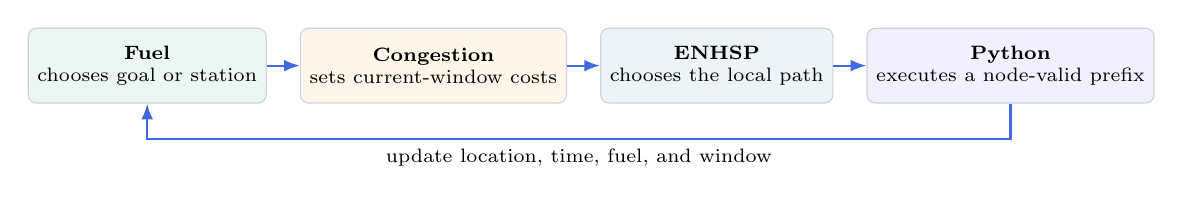
\begin{tikzpicture}[
    node distance=0.42cm,
    box/.style={draw=RoutlyRule,rounded corners=3pt,minimum height=0.95cm,minimum width=2.38cm,align=center,font=\scriptsize},
    arr/.style={-{Latex[length=2mm]},thick,draw=RoutlyBlue}
  ]
    \node[box,fill=RoutlyPaleGreen] (fuel) {\textbf{Fuel}\\chooses goal or station};
    \node[box,right=of fuel,fill=RoutlyPaleOrange] (cong) {\textbf{Congestion}\\sets current-window costs};
    \node[box,right=of cong,fill=RoutlyPaleBlue] (plan) {\textbf{ENHSP}\\chooses the local path};
    \node[box,right=of plan,fill=RoutlyPalePurple] (python) {\textbf{Python}\\executes a node-valid prefix};
    \draw[arr] (fuel) -- (cong);
    \draw[arr] (cong) -- (plan);
    \draw[arr] (plan) -- (python);
    \draw[arr] (python.south) -- ++(0,-0.45) -| node[pos=0.25,below,font=\scriptsize] {update location, time, fuel, and window} (fuel.south);
  \end{tikzpicture}

  \vspace{0.48cm}
  \begin{columns}[T,onlytextwidth]
    \begin{column}{0.32\textwidth}
      \metric{metric purple}{Online events}{inject disruptions after partial route execution}
    \end{column}
    \begin{column}{0.32\textwidth}
      \metric{metric blue}{More cities}{test grid, radial, and irregular topologies}
    \end{column}
    \begin{column}{0.32\textwidth}
      \metric{metric orange}{Stronger baselines}{larger LLM pool and geometric/time-dependent comparisons}
    \end{column}
  \end{columns}

  \vspace{0.35cm}
  \centering
  \textbf{Fuel chooses the target. Congestion chooses the costs. ENHSP chooses the path. Python updates the state.}
  \note{Time: 35 seconds. Describe the joint controller as a strict hierarchy. Fuel decides whether the next target is the final goal or a reachable station. Congestion supplies costs for the current time window. ENHSP finds the local route, and Python executes a node-consistent prefix before updating all state variables. Add online events, other cities, and stronger baselines.}
\end{frame}

% 18 --------------------------------------------------------------------------
\begin{frame}[plain]
  \centering
  \vspace{1.25cm}
  {\Huge\bfseries Thank you!\par}
  \vspace{0.18cm}
  {\Large Questions?\par}

  \vspace{0.65cm}
  {\normalsize Source code and reproducible configuration are available on GitHub:}\par
  \vspace{0.18cm}
  \href{https://github.com/GiuseppeRudi/routly-planner}{\color{RoutlyBlue}\Large\texttt{GiuseppeRudi/routly-planner}}

  \vspace{0.75cm}
  
\begin{tikzpicture}
    \draw[very thick,RoutlyBlue] (0,0) -- (2.5,0);
    \draw[very thick,RoutlyPurple] (2.5,0) -- (5.0,0);
    \draw[very thick,RoutlyMagenta] (5.0,0) -- (7.5,0);
  \end{tikzpicture}
  \note{Time: 15 seconds. Thank the audience, invite questions, and point to the repository for source code, configuration snapshots, and reproducible experiment artifacts.}
\end{frame}

\end{document}
